% Compile with XeLaTeX or Tectonic: tectonic Small-GPT-Project-Document.tex
\documentclass[11pt,a4paper]{article}
\usepackage{iftex}
\ifPDFTeX
  \usepackage[utf8]{inputenc}
  \usepackage[T1]{fontenc}
  \usepackage{lmodern}
\else
  \usepackage{fontspec}
\fi
\usepackage[margin=2.4cm]{geometry}
\usepackage{amsmath,amssymb}
\usepackage{microtype}
\usepackage{parskip}
\usepackage{graphicx}
\usepackage{float}
\usepackage[font=small,labelfont=bf]{caption}
\usepackage{array,booktabs,longtable}
\usepackage{xcolor}
\usepackage{listings}
\usepackage{needspace}
\usepackage[colorlinks=true,linkcolor=black,urlcolor=blue!55!black]{hyperref}

\definecolor{codebg}{gray}{0.965}
\definecolor{coderule}{gray}{0.82}
\lstset{
  basicstyle=\ttfamily\footnotesize,
  backgroundcolor=\color{codebg},
  frame=single,
  rulecolor=\color{coderule},
  framesep=5pt,
  xleftmargin=6pt,
  xrightmargin=6pt,
  columns=fullflexible,
  keepspaces=true,
  upquote=true,
  breaklines=true,
  breakindent=18pt,
  showstringspaces=false,
  keywordstyle=\color{blue!60!black},
  commentstyle=\color{black!55},
  stringstyle=\color{green!35!black},
  aboveskip=8pt,
  belowskip=8pt,
}
\setcounter{tocdepth}{1}
\setlength{\LTpre}{6pt}
\setlength{\LTpost}{8pt}
\newcommand{\vs}{\textvisiblespace}
\newcommand{\code}[1]{\texttt{#1}}
\raggedbottom

\title{Small-GPT\\Project Document}
\author{}
\date{6 November 2026}

\begin{document}
\maketitle


\tableofcontents
\newpage

\section*{Summary}
\phantomsection
\addcontentsline{toc}{section}{Summary}

Small-GPT now has a 185M-parameter story model, trained from scratch on one RTX 3060. It beats the earlier 24M model on both held-out test sets. Its short children's stories mostly hold together: in a 40-story test, 37 ended on their own and about 12 had a clear slip in logic or names.

{\small
\begin{longtable}{@{}>{\raggedright\arraybackslash\hspace{0pt}}p{\dimexpr 0.144\linewidth-2\tabcolsep\relax}>{\raggedright\arraybackslash\hspace{0pt}}p{\dimexpr 0.171\linewidth-2\tabcolsep\relax}>{\raggedright\arraybackslash\hspace{0pt}}p{\dimexpr 0.279\linewidth-2\tabcolsep\relax}>{\raggedright\arraybackslash\hspace{0pt}}p{\dimexpr 0.190\linewidth-2\tabcolsep\relax}>{\raggedright\arraybackslash\hspace{0pt}}p{\dimexpr 0.217\linewidth-2\tabcolsep\relax}@{}}
\toprule
\textbf{Model} & \textbf{Parameters} & \textbf{Training text} & \textbf{TinyStories test, bits/char} & \textbf{SimpleStories test, bits/char} \\
\midrule
\endhead
v2, served by the app today & 24.1M & TinyStories, 556M tokens, 2 passes & 0.408 & 1.041 \\
v3, new & 184.6M & TinyStories + SimpleStories, 1.15B tokens, 2 passes & \textbf{0.348} & \textbf{0.450} \\
\bottomrule
\end{longtable}
}

Lower is better. Bits per character is the fair yardstick here because the two models use different tokenizers.

\begin{itemize}
\item v3 trained for 93,400 steps, about 2.3B tokens, in about 60 hours of GPU time from 3 to 5 November 2026.
\item Two pauses and two power cuts hit the run. Each cut lost at most 5 minutes of training, because checkpoints are written whole and the run resumes from them.
\item It is a story writer, not an assistant. Asked “What is the capital of France?”, it writes a story.
\item The web app still serves v2. Switching it to v3 is a one-line change, waiting on a decision.
\end{itemize}

\section*{Goal and approach}
\phantomsection
\addcontentsline{toc}{section}{Goal and approach}

The goal is to build a language model from scratch and prove that the whole pipeline works on a home GPU. Stories were chosen because a small model can learn them well enough to judge by reading.

The project began as an educational codebase trained on an essay corpus. On 2 November 2026 that corpus was measured and found too small for coherent text:

\begin{itemize}
\item 752 sources, all unreviewed synthetic text from \code{gpt-\allowbreak{}oss:120b-\allowbreak{}cloud}, about 1.4M training tokens.
\item The best 16M model reached validation loss 5.43 (perplexity 227), and its samples were incoherent.
\item The 100M profile memorized the training set: train loss 0.04, validation loss 8.08.
\end{itemize}

Two routes were offered: connect retrieval to a pretrained model, or build from scratch on better data. The choice was \textbf{build from scratch}, in three steps:

\begin{enumerate}
\item Prove the pipeline on TinyStories, a public set of simple stories with a known good result for small models.
\item Grow the model while the data allows it, checking held-out loss and samples at each step.
\item Add more story data and use most of the GPU's 12 GB, to get the best story model the machine can train.
\end{enumerate}

For the last step, three sizes were measured on the real trainer: 94M, 140M and 185M parameters. 140M was recommended as the safer fit. The choice was 185M, which uses about 10.9 GB of GPU memory, and it fit.

\section*{Repository tour}
\phantomsection
\addcontentsline{toc}{section}{Repository tour}

The code is about 5,200 lines of Python in nine folders, with 55 unit tests. Text flows from \code{dataset/\allowbreak{}} through \code{tokenizer/\allowbreak{}} into \code{training/\allowbreak{}}, and the checkpoints it writes feed \code{evaluation.\allowbreak{}py}, \code{generation/\allowbreak{}} and \code{web/\allowbreak{}}.

{\small
\begin{longtable}{@{}>{\raggedright\arraybackslash\hspace{0pt}}p{\dimexpr 0.321\linewidth-2\tabcolsep\relax}>{\raggedright\arraybackslash\hspace{0pt}}p{\dimexpr 0.140\linewidth-2\tabcolsep\relax}>{\raggedright\arraybackslash\hspace{0pt}}p{\dimexpr 0.538\linewidth-2\tabcolsep\relax}@{}}
\toprule
\textbf{Path} & \textbf{Lines} & \textbf{What it does} \\
\midrule
\endhead
\code{dataset/\allowbreak{}engine.\allowbreak{}py} & 556 & Small-corpus pipeline: reads PDF, TXT and HTML, cleans and deduplicates, splits by source, writes token binaries \\
\code{dataset/\allowbreak{}large\_\allowbreak{}text.\allowbreak{}py} & 133 & Streams multi-gigabyte text files from disk, trains the tokenizer, writes \code{train.\allowbreak{}bin} and \code{val.\allowbreak{}bin} with EOS after each story \\
\code{tokenizer/\allowbreak{}bpe.\allowbreak{}py} & 973 & Byte-pair tokenizer, with a word-level mode for large text and an EOS token \\
\code{model/\allowbreak{}modern\_\allowbreak{}gpt.\allowbreak{}py} & 838 & The Transformer: RMSNorm, RoPE, grouped-query attention, SwiGLU, tied embeddings, sampling \\
\code{model/\allowbreak{}count.\allowbreak{}py} & 89 & Counts parameters for a profile \\
\code{training/\allowbreak{}config.\allowbreak{}py} & 83 & Size profiles and optimizer settings \\
\code{training/\allowbreak{}train.\allowbreak{}py} & 584 & Training in three modes: new, resume, and update with replay; atomic checkpoints \\
\code{evaluation.\allowbreak{}py} & 217 & Fixed-window held-out loss with data and tokenizer hashes, saved as JSON \\
\code{generation/\allowbreak{}generate.\allowbreak{}py} & 112 & Command-line text generation from a checkpoint \\
\code{web/\allowbreak{}server.\allowbreak{}py}, \code{web/\allowbreak{}app.\allowbreak{}js} & 281, 390 & Local web app for trying a model in the browser \\
\code{rag.\allowbreak{}py} & 101 & Lexical retrieval over source chunks, used with the essay model \\
\code{pipeline/\allowbreak{}learn.\allowbreak{}py} & 121 & Rebuilds topic data with a fixed tokenizer and runs a replay update \\
\code{generate\_\allowbreak{}text.\allowbreak{}py} & 128 & Makes synthetic lessons with an Ollama model; the source of the old essay corpus \\
\code{experiments/\allowbreak{}benchmark.\allowbreak{}py} & 43 & Repeatable validation perplexity with run metadata \\
\code{tests/\allowbreak{}} & 948 & Tests for data, tokenizer, model, training, retrieval and large-text builds \\
\bottomrule
\end{longtable}
}

The story runs also used scripts in \code{reports/\allowbreak{}}, which stays out of git because it holds local paths. The Appendix lists them.

\section*{Hardware and software}
\phantomsection
\addcontentsline{toc}{section}{Hardware and software}

Everything ran on one desktop PC, with no cloud compute.

{\small
\begin{longtable}{@{}>{\raggedright\arraybackslash\hspace{0pt}}p{\dimexpr 0.199\linewidth-2\tabcolsep\relax}>{\raggedright\arraybackslash\hspace{0pt}}p{\dimexpr 0.801\linewidth-2\tabcolsep\relax}@{}}
\toprule
\textbf{Part} & \textbf{What was used} \\
\midrule
\endhead
GPU & NVIDIA GeForce RTX 3060, 12 GB, 170 W power limit, driver 580.178.04 \\
CPU & AMD Ryzen 5 7600, 6 cores, 12 threads \\
Memory & 30 GiB \\
Disk & Ramsta S800 240 GB SATA SSD for the system, code, data and checkpoints; about 15 GB free at the end \\
System & Ubuntu 24.04.4, Linux kernel 7.0.0-38, then 7.0.0-42 after a reboot \\
Software & Python 3.12.14, PyTorch 2.14.0 with CUDA 13.0, NumPy 2.5.2, in a conda environment \\
\bottomrule
\end{longtable}
}

During the 185M run the GPU sat at 100\% load, 160-163 W and 66-71°C, without thermal throttling. The CPU stayed near 70°C and the SSD near 50°C. The PC has two more NVMe drives, but they hold Windows partitions and were not needed: training speed depends on the GPU, not the disk.

\section*{Data}
\phantomsection
\addcontentsline{toc}{section}{Data}

The final model trained on 1.15 billion tokens of children's stories from two public datasets, about 800 times more text than the essay corpus. Only counts and hashes were inspected; the story text itself was not read.

{\small
\begin{longtable}{@{}>{\raggedright\arraybackslash\hspace{0pt}}p{\dimexpr 0.185\linewidth-2\tabcolsep\relax}>{\raggedright\arraybackslash\hspace{0pt}}p{\dimexpr 0.391\linewidth-2\tabcolsep\relax}>{\raggedright\arraybackslash\hspace{0pt}}p{\dimexpr 0.140\linewidth-2\tabcolsep\relax}>{\raggedright\arraybackslash\hspace{0pt}}p{\dimexpr 0.192\linewidth-2\tabcolsep\relax}>{\raggedright\arraybackslash\hspace{0pt}}p{\dimexpr 0.092\linewidth-2\tabcolsep\relax}@{}}
\toprule
\textbf{Data set} & \textbf{Source and licence} & \textbf{Stories} & \textbf{Tokens} & \textbf{Used for} \\
\midrule
\endhead
Essay corpus & 752 synthetic lessons from \code{gpt-\allowbreak{}oss:120b-\allowbreak{}cloud}, unreviewed & 752 sources & 1.41M train, 54K val & Early 16M and 100M runs \\
TinyStories V2 (GPT-4 stories) & \href{https://huggingface.co/datasets/roneneldan/TinyStories}{roneneldan/TinyStories}, CDLA-Sharing-1.0 & 2,717,495 train, 27,630 valid & 556M train, 5.6M val (vocab 4096) & v1, v2 and v3 \\
SimpleStories & \href{https://huggingface.co/datasets/SimpleStories/SimpleStories}{SimpleStories/SimpleStories}, MIT & 2,115,669 train, 21,371 test & Part of v3's total below & v3 \\
stories-v3, combined & Built by \code{reports/\allowbreak{}make\_\allowbreak{}stories\_\allowbreak{}text.\allowbreak{}py} & 4,833,164 train, 49,001 val & 1,147,643,766 train, 11,590,840 val (vocab 8192) & v3 \\
\bottomrule
\end{longtable}
}

How the combined set was built:

\begin{enumerate}
\item The SimpleStories test split was written first, as \code{simple-\allowbreak{}test.\allowbreak{}txt}, with blank and repeated stories skipped.
\item Training text = all TinyStories training stories, then the SimpleStories training stories. 25 repeated stories and 2 stories identical to a test story were dropped.
\item Validation text = the TinyStories validation file plus \code{simple-\allowbreak{}test.\allowbreak{}txt}, so neither test set is in training.
\item \code{dataset.\allowbreak{}large\_\allowbreak{}text} trained an 8192-token tokenizer on the training text and wrote \code{train.\allowbreak{}bin} and \code{val.\allowbreak{}bin}, with an end-of-story (EOS) token after every story.
\end{enumerate}

The tokenizer is word-level BPE: merges never cross a space, so no token spans two words. Each v3 token covers 4.18 characters of validation text on average, against 3.93 for the 4096-token v2 tokenizer. 115 of the 8192 tokens never appear in training.

Every data folder has a \code{meta.\allowbreak{}json} with SHA-256 hashes of its files. The trainer refuses to start if the data or tokenizer no longer match the checkpoint, which caught nothing in this project, but made each power-cut check quick.

\section*{Model}
\phantomsection
\addcontentsline{toc}{section}{Model}

All runs use the same decoder-only Transformer in \code{model/\allowbreak{}modern\_\allowbreak{}gpt.\allowbreak{}py}; only its size changes. Each block applies RMSNorm, then causal grouped-query attention with rotary position embeddings (RoPE), then RMSNorm and a SwiGLU feed-forward layer, each with a residual connection. The output layer shares its weights with the token embedding.

{\footnotesize
\begin{longtable}{@{}>{\raggedright\arraybackslash\hspace{0pt}}p{\dimexpr 0.131\linewidth-2\tabcolsep\relax}>{\raggedright\arraybackslash\hspace{0pt}}p{\dimexpr 0.098\linewidth-2\tabcolsep\relax}>{\raggedright\arraybackslash\hspace{0pt}}p{\dimexpr 0.107\linewidth-2\tabcolsep\relax}>{\raggedright\arraybackslash\hspace{0pt}}p{\dimexpr 0.101\linewidth-2\tabcolsep\relax}>{\raggedright\arraybackslash\hspace{0pt}}p{\dimexpr 0.123\linewidth-2\tabcolsep\relax}>{\raggedright\arraybackslash\hspace{0pt}}p{\dimexpr 0.226\linewidth-2\tabcolsep\relax}>{\raggedright\arraybackslash\hspace{0pt}}p{\dimexpr 0.214\linewidth-2\tabcolsep\relax}@{}}
\toprule
\textbf{Profile} & \textbf{Width} & \textbf{Layers} & \textbf{Query / KV heads} & \textbf{Feed-forward} & \textbf{Parameters} & \textbf{Trained as} \\
\midrule
\endhead
\code{small} & 384 & 6 & 6 / 2 & 1024 & 15.7M (vocab 16384), 11.0M (vocab 4096) & Essay runs, TinyStories v1 \\
\code{medium} & 512 & 8 & 8 / 2 & 1365 & 24.1M (vocab 4096) & TinyStories v2 \\
\code{3060} & 768 & 14 & 12 / 4 & 2048 & 100.7M (vocab 16384) & Old essay run that memorized its data \\
\code{large} & 1024 & 16 & 16 / 4 & 2730 & 184.6M (vocab 8192) & Stories v3 \\
\bottomrule
\end{longtable}
}

Every profile reads 768 tokens of context, uses dropout 0.1 (0.05 for \code{3060}), and takes its vocabulary size from the tokenizer. The parameter count of \code{large} adds up exactly:

\begin{itemize}
\item Token embedding, shared with the output layer: 8192 $\times$ 1024 = 8,388,608.
\item Each of 16 blocks: attention 2,621,440 (query and output 1024 $\times$ 1024 each, key and value 1024 $\times$ 256 each), SwiGLU 8,386,560 (three 1024 $\times$ 2730 matrices), two norms 2,048. That is 11,010,048 per block.
\item Final norm: 1,024. Total: 184,550,400.
\end{itemize}

Grouped-query attention lets 16 query heads share 4 key/value heads, which cuts the key and value weights by three quarters. Generation samples with temperature, top-k, top-p and a repetition penalty. It recomputes the full context for each new token, with no key/value cache.

\section*{Training setup}
\phantomsection
\addcontentsline{toc}{section}{Training setup}

Every story run used the same recipe: next-token prediction on random 768-token windows, 24,576 tokens per optimizer step, and AdamW with a warmup and cosine schedule. Only the model size, the data and the number of steps changed.

{\small
\begin{longtable}{@{}>{\raggedright\arraybackslash\hspace{0pt}}p{\dimexpr 0.299\linewidth-2\tabcolsep\relax}>{\raggedright\arraybackslash\hspace{0pt}}p{\dimexpr 0.701\linewidth-2\tabcolsep\relax}@{}}
\toprule
\textbf{Setting} & \textbf{Value} \\
\midrule
\endhead
Batch & 8 windows $\times$ 4 accumulation steps $\times$ 768 tokens = 24,576 tokens per step \\
Optimizer & AdamW, betas 0.9 and 0.95, weight decay 0.1 (not on norms or the shared embedding) \\
Learning rate & Peak 3e-4, linear warmup over 150 steps, cosine decay to a floor of 3e-5 \\
Gradient clipping & Norm 1.0 \\
Precision & float16 autocast with a gradient scaler \\
Evaluation & Every 500 steps, 20 random validation batches \\
Checkpoints & \code{gpt-\allowbreak{}best.\allowbreak{}pt} at the lowest validation loss, \code{gpt.\allowbreak{}pt} at every evaluation \\
\bottomrule
\end{longtable}
}

The targets are the input window shifted by one token, so the model learns to predict each next token from the ones before it. Validation loss drives the choice of best checkpoint.

A 185M checkpoint is 2.2 GB, about 12 bytes per parameter: 4 for the weights and 8 for AdamW's two moment estimates. Each file is first written to a temporary name, then renamed into place. A power cut can therefore lose the newest steps, but never leave a half-written checkpoint.

\code{-\allowbreak{}-\allowbreak{}mode resume} restores the weights, optimizer state, random-number state and the planned schedule. It then continues to the planned final step as if nothing had happened. The trainer also checks the data and tokenizer hashes against the checkpoint before it starts.

\section*{Run history}
\phantomsection
\addcontentsline{toc}{section}{Run history}

Six full runs led to the final model. Each story run beat its own data's simple baseline by a wider margin than the one before.

{\small
\begin{longtable}{@{}>{\raggedright\arraybackslash\hspace{0pt}}p{\dimexpr 0.103\linewidth-2\tabcolsep\relax}>{\raggedright\arraybackslash\hspace{0pt}}p{\dimexpr 0.167\linewidth-2\tabcolsep\relax}>{\raggedright\arraybackslash\hspace{0pt}}p{\dimexpr 0.209\linewidth-2\tabcolsep\relax}>{\raggedright\arraybackslash\hspace{0pt}}p{\dimexpr 0.161\linewidth-2\tabcolsep\relax}>{\raggedright\arraybackslash\hspace{0pt}}p{\dimexpr 0.163\linewidth-2\tabcolsep\relax}>{\raggedright\arraybackslash\hspace{0pt}}p{\dimexpr 0.197\linewidth-2\tabcolsep\relax}@{}}
\toprule
\textbf{Dates} & \textbf{Run} & \textbf{Data} & \textbf{Steps (passes), time} & \textbf{Validation loss} & \textbf{Perplexity, and times lower than a bigram baseline} \\
\midrule
\endhead
3-5 Nov 2026 & \code{stories-\allowbreak{}v3}, 184.6M & TinyStories + SimpleStories, vocab 8192 & 93,400 (2.0), about 60 h & 1.170 & 3.2, 23$\times$ lower \\
3 Nov 2026 & \code{tinystories-\allowbreak{}v2}, 24.1M & TinyStories, vocab 4096 & 45,000 (2.0), 5.9 h & 1.110 & 3.0, 18$\times$ lower \\
2 Nov 2026 & \code{tinystories-\allowbreak{}v1}, 11.0M & TinyStories, vocab 4096 & 20,000 (0.88), 1.4 h & 1.282 & 3.6, 15$\times$ lower \\
2 Nov 2026 & \code{small-\allowbreak{}v2} (essays), 15.7M & Essay corpus, vocab 16384 & best at 1,699 of 3,000 & 5.43 & 227, 4.6$\times$ lower \\
2 Nov 2026 & \code{small-\allowbreak{}v1} (essays), 15.7M & Essay corpus, vocab 16384 & 1,500 & 5.63 & 279 \\
Before Nov 2026 & \code{100m-\allowbreak{}v1} (essays), 100.7M & Essay corpus, vocab 16384 & best at 999 of 5,000 & 5.73 & 308; train loss fell to 0.04 by the end \\
\bottomrule
\end{longtable}
}

Validation losses are full passes over each run's own validation set. They compare only within the same data and tokenizer, so v3's 1.170 is not worse than v2's 1.110; the Final results section compares them fairly.

What each step taught:

\begin{itemize}
\item \textbf{Essay runs.} The data, not the model, was the limit. Validation loss bottomed out at step 1,700, then rose as the model memorized.
\item \textbf{v1.} The pipeline works: on real story data an 11M model writes stories that end at EOS and almost never repeat themselves.
\item \textbf{v2.} Twice the parameters and two passes lowered validation loss from 1.282 to 1.110 on the same data. Validation rose at only 2 of 89 checks.
\item \textbf{v3.} With more data, a model 7.7 times larger keeps improving to its last step, with a small train-validation gap.
\end{itemize}

A 140M trial of v3's data was started and stopped after 4.5 minutes, once 185M was chosen.

\section*{Final results}
\phantomsection
\addcontentsline{toc}{section}{Final results}

v3 is the best model the project has trained. On TinyStories test text it scores 0.348 bits per character, 15\% below v2. On SimpleStories test text it scores 0.450, 57\% below v2.

Each model read both test texts with its own tokenizer, in 768-token windows:

{\footnotesize
\begin{longtable}{@{}>{\raggedright\arraybackslash\hspace{0pt}}p{\dimexpr 0.093\linewidth-2\tabcolsep\relax}>{\raggedright\arraybackslash\hspace{0pt}}p{\dimexpr 0.192\linewidth-2\tabcolsep\relax}>{\raggedright\arraybackslash\hspace{0pt}}p{\dimexpr 0.136\linewidth-2\tabcolsep\relax}>{\raggedright\arraybackslash\hspace{0pt}}p{\dimexpr 0.161\linewidth-2\tabcolsep\relax}>{\raggedright\arraybackslash\hspace{0pt}}p{\dimexpr 0.100\linewidth-2\tabcolsep\relax}>{\raggedright\arraybackslash\hspace{0pt}}p{\dimexpr 0.161\linewidth-2\tabcolsep\relax}>{\raggedright\arraybackslash\hspace{0pt}}p{\dimexpr 0.155\linewidth-2\tabcolsep\relax}@{}}
\toprule
\textbf{Model} & \textbf{Test text} & \textbf{Tokens} & \textbf{Characters per token} & \textbf{Loss, nats per token} & \textbf{Perplexity} & \textbf{Bits per character} \\
\midrule
\endhead
v2 & TinyStories valid & 5,617,373 & 3.929 & 1.1098 & 3.03 & 0.4076 \\
v3 & TinyStories valid & 5,478,455 & 4.028 & 0.9728 & 2.65 & \textbf{0.3484} \\
v2 & SimpleStories test & 7,042,723 & 3.753 & 2.7071 & 14.99 & 1.0407 \\
v3 & SimpleStories test & 6,112,385 & 4.324 & 1.3472 & 3.85 & \textbf{0.4495} \\
\bottomrule
\end{longtable}
}

Loss per token rewards a tokenizer with longer tokens, so it cannot compare these two models. Bits per character divides that out:
\[
\text{bits per character} = \frac{\text{loss per token (nats)}}{\text{characters per token} \times \ln 2}
\]

Decoding the tokens gave back exactly the 22,067,904 and 26,430,797 characters of the two texts, so neither tokenizer drops text.

How to read the two rows:

\begin{itemize}
\item \textbf{TinyStories is the like-for-like test.} Both models trained on the same TinyStories training text; v3 also had SimpleStories and 7.7 times the parameters.
\item \textbf{SimpleStories mostly shows what the new data added.} v2 never saw that style, so its 1.041 is expected.
\item \textbf{One caveat.} \code{simple-\allowbreak{}test.\allowbreak{}txt} is half of v3's validation set, so it helped pick the best checkpoint. That choice was between near-equal steps: the best (92,499) and last (93,399) differ by 0.0007 in validation loss. No test story was trained on.
\end{itemize}

Neither model memorized its data. Measured with dropout off on 2,000 random windows each:

{\small
\begin{longtable}{@{}>{\raggedright\arraybackslash\hspace{0pt}}p{\dimexpr 0.126\linewidth-2\tabcolsep\relax}>{\raggedright\arraybackslash\hspace{0pt}}p{\dimexpr 0.233\linewidth-2\tabcolsep\relax}>{\raggedright\arraybackslash\hspace{0pt}}p{\dimexpr 0.260\linewidth-2\tabcolsep\relax}>{\raggedright\arraybackslash\hspace{0pt}}p{\dimexpr 0.166\linewidth-2\tabcolsep\relax}>{\raggedright\arraybackslash\hspace{0pt}}p{\dimexpr 0.213\linewidth-2\tabcolsep\relax}@{}}
\toprule
\textbf{Model} & \textbf{Training loss} & \textbf{Validation loss} & \textbf{Gap} & \textbf{Unique training tokens per parameter} \\
\midrule
\endhead
v2 & 1.0955 & 1.1115 & 0.016 & 23.1 \\
v3 & 1.1286 & 1.1623 & 0.034 & 6.2 \\
\bottomrule
\end{longtable}
}

v3's gap is twice v2's because it has far fewer training tokens per parameter, but 0.034 is still small. Over its full validation set, v3 scores 1.1702 nats per token (perplexity 3.22), against 4.30 (perplexity 73.7) for a bigram baseline built from its training text.

The training curve has a long, slow tail. Validation loss fell by 1.034 in the first 10,000 steps, by 0.235 over the next 40,000, and by 0.092 over the last 43,400. It rose at 16 of 187 checks, never by more than 0.0012.

\begin{figure}[H]
\centering
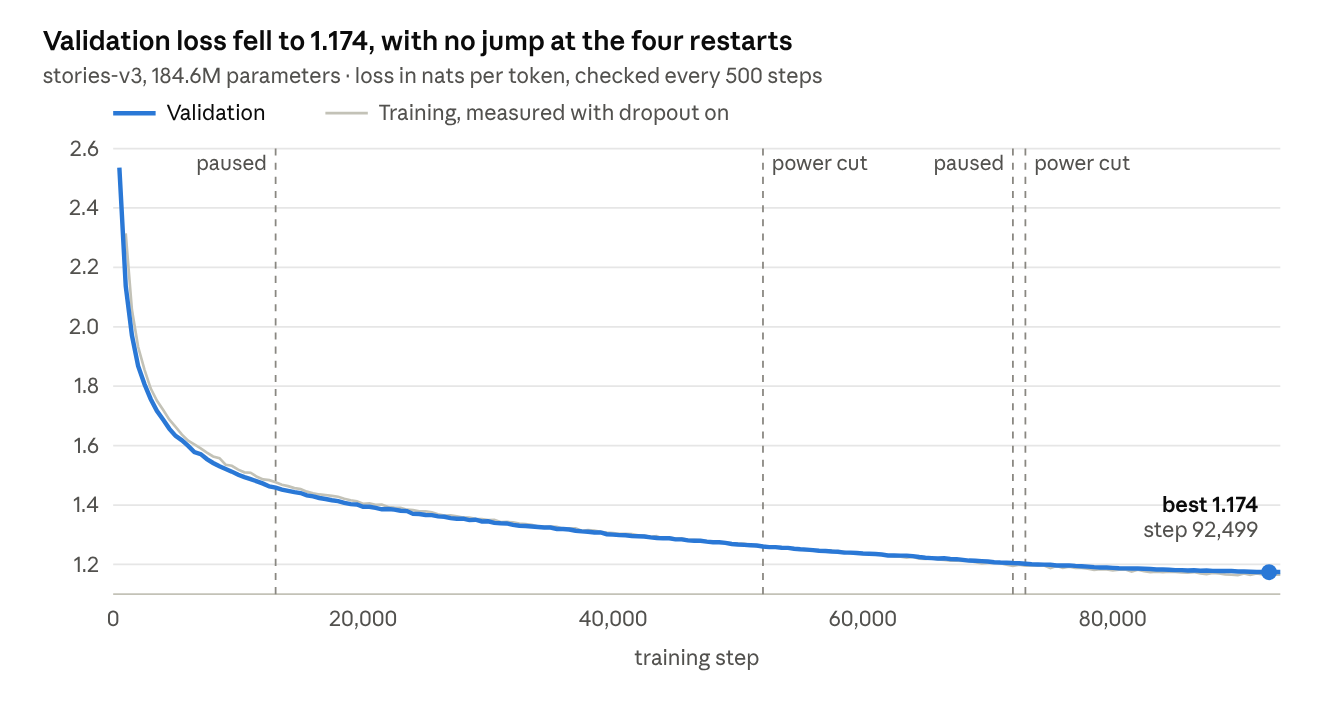
\includegraphics[width=\linewidth]{small-gpt-project-figures/v3-loss-curve.png}
\caption{reports/stories-v3-train.log $\cdot$ 187 checks, steps 499 to 93,399}
\end{figure}

The grey training line sits slightly above validation for much of the run because it is measured with dropout on; measured with dropout off, training loss is lower, as the gap table shows.

The \code{reports/\allowbreak{}stories-\allowbreak{}v3.\allowbreak{}json} file written at the end says 1.1246. That figure comes from only 200 windows, 1.3\% of the validation text, which mixes two styles with very different losses. Quote the full pass instead.

\section*{Story quality}
\phantomsection
\addcontentsline{toc}{section}{Story quality}

v3's stories hold together more often than v2's, but both make the same kinds of mistakes. Reading 40 stories from each, I counted a clear slip in logic or names in about 12 of v3's, against about 19 of v2's.

Both models got 8 new story openings, 5 random seeds each, at the app's settings. None of these openings was used to choose or score a model.

{\small
\begin{longtable}{@{}>{\raggedright\arraybackslash\hspace{0pt}}p{\dimexpr 0.612\linewidth-2\tabcolsep\relax}>{\raggedright\arraybackslash\hspace{0pt}}p{\dimexpr 0.188\linewidth-2\tabcolsep\relax}>{\raggedright\arraybackslash\hspace{0pt}}p{\dimexpr 0.201\linewidth-2\tabcolsep\relax}@{}}
\toprule
\textbf{Measure} & \textbf{v2 (24M)} & \textbf{v3 (185M)} \\
\midrule
\endhead
Stories that ended on their own & 40 of 40 & 37 of 40 \\
Average length, tokens & 145 & 154 \\
Repeated 4-word phrases within a story & 0.7\% & 0.5\% \\
Made-up words, against 24,255 words seen in the data & 0 of 4,607 & 0 of 4,973 \\
16-token runs also found in v3's training text & 4.9\% & 4.4\% \\
Stories with a clear slip, by one reader & about 19 & about 12 \\
\bottomrule
\end{longtable}
}

The copying check counts both models against v3's training text, which includes all of v2's. Under 5\% of runs match, mostly stock phrases such as “they became best friends”, so both models compose their stories rather than recite them.

What v3 does well: plain, correct sentences, punctuated dialogue, and a clear arc from problem to ending. A typical good one: “As Ben rowed, he saw a duck with a hurt wing... The duck thanked Ben and they became friends. The end.”

Where v3 still slips:

\begin{itemize}
\item \textbf{Names drift.} One story opens with Ben's boat, then turns into an argument between Tom and Sam. Another switches from Ben to Alex halfway through.
\item \textbf{Facts contradict.} “As the sun went down... They watched the beautiful sunrise.” A mouse says “Meow!”
\item \textbf{Twists don't follow.} A lady who finds her kitten takes off her hat and turns out to be Anna's dad.
\item \textbf{Some stories run long.} Three of 40 reached the 400-token limit, and two of those stopped mid-sentence.
\end{itemize}

v2's slips are more often nonsense: “The water turned into water!”, “I was a dog, but now I am a dog again”, and a toy train “with a track that went around the track”.

Neither model answers questions. Given “What is the capital of France?”, v3 wrote a story about two children and a man with a “cap case”. It also ran to the token limit. The other five fixed prompts all ended on their own.

\section*{Working through power cuts}
\phantomsection
\addcontentsline{toc}{section}{Working through power cuts}

Routine load shedding cut the power four times. The first killed a training run; after that, every long job was made resumable, and the next three cuts lost a few minutes of work at most.

{\small
\begin{longtable}{@{}>{\raggedright\arraybackslash\hspace{0pt}}p{\dimexpr 0.159\linewidth-2\tabcolsep\relax}>{\raggedright\arraybackslash\hspace{0pt}}p{\dimexpr 0.271\linewidth-2\tabcolsep\relax}>{\raggedright\arraybackslash\hspace{0pt}}p{\dimexpr 0.246\linewidth-2\tabcolsep\relax}>{\raggedright\arraybackslash\hspace{0pt}}p{\dimexpr 0.325\linewidth-2\tabcolsep\relax}@{}}
\toprule
\textbf{When} & \textbf{Event} & \textbf{Work lost} & \textbf{Recovery} \\
\midrule
\endhead
6 Nov, 00:15 to 09:10 & Power cut during final scoring & Two scoring steps not yet run & Finished logs were already saved in \code{reports/\allowbreak{}}; the two steps were rerun \\
5 Nov, about 10:00 to 10:14 & Power cut at about step 73,100 & About 5 minutes, since the save at step 72,999 & Data hashes and both checkpoints checked; resumed at 10:19 from step 73,000 \\
5 Nov, 09:00 to 09:16 & Planned pause right after the step 71,999 save & None & Resumed \\
4 Nov, 18:53 to 20:16 & Power cut & About 1 minute, since the save at step 51,999 & Checks passed; resumed at about 20:18. The reboot also moved the kernel from 7.0.0-38 to 7.0.0-42 \\
3 Nov, 18:05 to 18:15 & Planned pause right after the step 12,999 save & None & Resumed \\
2 Nov & Power cut killed an essay training run and wiped \code{/\allowbreak{}tmp} & The run, plus scripts and logs kept in \code{/\allowbreak{}tmp} & Led to the rules below \\
\bottomrule
\end{longtable}
}

The rules that made this work:

\begin{itemize}
\item \textbf{Write files whole.} Checkpoints and data builds go to a temporary name first, then get renamed into place.
\item \textbf{Keep logs in the project.} Logs and scoring scripts live in \code{reports/\allowbreak{}}, never in \code{/\allowbreak{}tmp}, which is wiped at boot.
\item \textbf{Flush log lines.} The trainer flushes each progress line, so a log written through \code{tee} keeps everything up to the cut.
\item \textbf{Check before resuming.} After each cut, the data files were hashed against \code{meta.\allowbreak{}json}, and both checkpoints were fully loaded and checked for invalid values.
\item \textbf{Pause on a save.} A planned stop waits for the next checkpoint, then sends an interrupt, so nothing is lost.
\end{itemize}

The training curve in Final results shows no jump at any of the four restarts.

\section*{Bugs found and fixed}
\phantomsection
\addcontentsline{toc}{section}{Bugs found and fixed}

The review on 2 November found that the app served a model which had memorized its data, plus a set of training and data bugs. They were fixed in \href{https://github.com/Jannatul-Naim/small-GPT-Model/pull/3}{PR 3}, with tests added at the same time.

{\small
\begin{longtable}{@{}>{\raggedright\arraybackslash\hspace{0pt}}p{\dimexpr 0.170\linewidth-2\tabcolsep\relax}>{\raggedright\arraybackslash\hspace{0pt}}p{\dimexpr 0.441\linewidth-2\tabcolsep\relax}>{\raggedright\arraybackslash\hspace{0pt}}p{\dimexpr 0.389\linewidth-2\tabcolsep\relax}@{}}
\toprule
\textbf{Area} & \textbf{Problem} & \textbf{Fix} \\
\midrule
\endhead
Serving & The app loaded the latest checkpoint, which had memorized its data (train 0.04, val 8.08) & Load \code{gpt-\allowbreak{}best.\allowbreak{}pt} \\
Serving & \code{python -\allowbreak{}m web.\allowbreak{}server}, the command in the README, did not start a server & Made it start one \\
Training & \code{-\allowbreak{}-\allowbreak{}mode new} could silently replace existing checkpoints & Refuse unless \code{-\allowbreak{}-\allowbreak{}overwrite}; add \code{-\allowbreak{}-\allowbreak{}checkpoint-\allowbreak{}dir} \\
Training & Resume restarted the warmup instead of continuing the schedule & Save the schedule in the checkpoint \\
Training & Updates could replace the best checkpoint with a worse one & Replace it only on a real improvement \\
Training & Weight decay hit the embedding and the norm scales & Skip decay on those \\
Data & Sources had no end marker, so generation never knew where to stop & EOS after each source; stop generation at EOS \\
Data & A prompt ending in a period could get an empty reply & Block EOS for the first 20 new tokens \\
Data & Three old scripts duplicated the engine and could leak validation text into training & Removed them \\
Tokenizer & A merge guard followed removed nodes through a negative index & Fixed the guard \\
Retrieval & Scores grew with repeated matches, and trailing punctuation created separate terms & Constant score per match; strip punctuation \\
\bottomrule
\end{longtable}
}

Later fixes came with the story work:

\begin{itemize}
\item The trainer now stops if the data files come from different builds (\href{https://github.com/Jannatul-Naim/small-GPT-Model/pull/4}{PR 4}).
\item The app applies the same repetition penalty as command-line generation, and its reply limit rose to 400 tokens so stories can finish (\href{https://github.com/Jannatul-Naim/small-GPT-Model/pull/4}{PR 4}).
\item Progress lines are flushed, so a log survives a power cut. This change is still uncommitted.
\end{itemize}

\section*{Web app}
\phantomsection
\addcontentsline{toc}{section}{Web app}

The web app is a local FastAPI server that streams a story continuation token by token at http://127.0.0.1:8000. It serves v2 by default; v3 runs with two extra options.

\Needspace{3\baselineskip}
\begin{lstlisting}
python -m web.server
\end{lstlisting}

\Needspace{3\baselineskip}
\begin{lstlisting}
python -m web.server --checkpoint checkpoints/stories-v3/gpt-best.pt --data-dir data/stories-v3
\end{lstlisting}

{\small
\begin{longtable}{@{}>{\raggedright\arraybackslash\hspace{0pt}}p{\dimexpr 0.338\linewidth-2\tabcolsep\relax}>{\raggedright\arraybackslash\hspace{0pt}}p{\dimexpr 0.662\linewidth-2\tabcolsep\relax}@{}}
\toprule
\textbf{Setting} & \textbf{Default} \\
\midrule
\endhead
Temperature & 0.75 \\
Top-k & 40 \\
Top-p & 0.92 \\
Repetition penalty & 1.08 \\
Reply limit & 400 tokens on the page; the server accepts up to 512 \\
Early stop & EOS is blocked for the first 20 new tokens \\
\bottomrule
\end{longtable}
}

With v2, 30 test replies through the app gave none blank and one that hit the 400-token limit (the France question), at 223 tokens per second. v3 was first run in the app on 6 November and wrote stories normally, but its speed has not been measured. Retrieval over source chunks still works with the old essay model, through \code{-\allowbreak{}-\allowbreak{}chunks}; the story models run without it. The app does not restart by itself after a reboot.

\section*{How to reproduce}
\phantomsection
\addcontentsline{toc}{section}{How to reproduce}

These are the commands that built and trained v3, run from the project folder. The build and the tests take minutes; training takes about 60 hours on an RTX 3060.

\begin{enumerate}
\item Download the source files into their own folders. Put \code{TinyStoriesV2-\allowbreak{}GPT4-\allowbreak{}train.\allowbreak{}txt} and \code{TinyStoriesV2-\allowbreak{}GPT4-\allowbreak{}valid.\allowbreak{}txt} from \href{https://huggingface.co/datasets/roneneldan/TinyStories}{roneneldan/TinyStories} in \code{data/\allowbreak{}tinystories/\allowbreak{}raw/\allowbreak{}}. Put the seven \code{train-\allowbreak{}*.\allowbreak{}parquet} files and \code{test-\allowbreak{}00000-\allowbreak{}of-\allowbreak{}00001.\allowbreak{}parquet} from \href{https://huggingface.co/datasets/SimpleStories/SimpleStories}{SimpleStories/SimpleStories} in \code{data/\allowbreak{}simplestories/\allowbreak{}raw/\allowbreak{}}.
\item Combine them into three text files. Run it with \code{-\allowbreak{}I}, because it reads downloaded files:
\end{enumerate}

\Needspace{3\baselineskip}
\begin{lstlisting}
python -I reports/make_stories_text.py
\end{lstlisting}

\begin{enumerate}
\setcounter{enumi}{2}
\item Train the tokenizer and write the token files:
\end{enumerate}

\Needspace{3\baselineskip}
\begin{lstlisting}
python -m dataset.large_text --train data/stories-v3/raw/train.txt --val data/stories-v3/raw/val.txt --out data/stories-v3 --vocab-size 8192
\end{lstlisting}

\begin{enumerate}
\setcounter{enumi}{3}
\item Train, keeping a log in \code{reports/\allowbreak{}}:
\end{enumerate}

\Needspace{3\baselineskip}
\begin{lstlisting}
python -m training.train --mode new --model-size large --steps 93400 --eval-interval 500 --data-dir data/stories-v3 --checkpoint-dir checkpoints/stories-v3 2>&1 | tee reports/stories-v3-train.log
\end{lstlisting}

\begin{enumerate}
\setcounter{enumi}{4}
\item After any stop or power cut, resume with the same folders:
\end{enumerate}

\Needspace{3\baselineskip}
\begin{lstlisting}
python -m training.train --mode resume --eval-interval 500 --data-dir data/stories-v3 --checkpoint-dir checkpoints/stories-v3 2>&1 | tee -a reports/stories-v3-train.log
\end{lstlisting}

\begin{enumerate}
\setcounter{enumi}{5}
\item Score the result:
\end{enumerate}

\Needspace{3\baselineskip}
\begin{lstlisting}
python reports/eval_stories.py checkpoints/stories-v3 data/stories-v3 best
\end{lstlisting}

\Needspace{3\baselineskip}
\begin{lstlisting}
python reports/score_bits.py
\end{lstlisting}

\Needspace{3\baselineskip}
\begin{lstlisting}
python reports/compare_stories.py checkpoints/tinystories-v2=data/tinystories checkpoints/stories-v3=data/stories-v3
\end{lstlisting}

\begin{enumerate}
\setcounter{enumi}{6}
\item Run the unit tests. All 55 pass in about 11 seconds on the CPU:
\end{enumerate}

\Needspace{3\baselineskip}
\begin{lstlisting}
python -m unittest discover -s tests
\end{lstlisting}

The \code{large} profile and the logging fix are still uncommitted, and \code{reports/\allowbreak{}} is not in git. Until they are committed, step 4 works only on this computer.

\section*{Limitations and honest claims}
\phantomsection
\addcontentsline{toc}{section}{Limitations and honest claims}

The evidence supports one claim: on this hardware, this code trains a model that writes simple children's stories well, and bigger models with more story data do measurably better. It does not support claims beyond that.

\begin{itemize}
\item \textbf{One genre.} Both datasets are synthetic children's stories written by other language models. The model has not been tested on any other kind of text.
\item \textbf{Not an assistant.} It continues text. It was never trained on questions and answers, so it cannot answer them.
\item \textbf{One run per size.} Every result comes from a single training run with one seed, so the run-to-run spread is unknown.
\item \textbf{Two test sets.} Both are held out from training, but \code{simple-\allowbreak{}test.\allowbreak{}txt} also helped choose v3's best step.
\item \textbf{Story quality is judged by reading and simple counts.} Stopping, repeated phrases, unknown words and copied 16-token runs are proxies; they miss logic slips.
\item \textbf{Under-trained by common rules of thumb.} v3 had 6.2 unique training tokens per parameter, well under the roughly 20 that compute-optimal training suggests. Its curve was still falling slowly at the end.
\item \textbf{Speed in the app is unmeasured} for v3.
\item \textbf{Single copies.} The checkpoints exist only on this PC's SSD, and the \code{large} profile and scoring scripts are not in git.
\end{itemize}

\section*{Next steps}
\phantomsection
\addcontentsline{toc}{section}{Next steps}

The first two steps protect what exists; the rest are choices about where to take the model.

\begin{itemize}
\item[$\square$] Commit the \code{large} profile, the logging fix and the scoring scripts on a new branch, without the local paths in \code{reports/\allowbreak{}}.
\item[$\square$] Copy \code{checkpoints/\allowbreak{}stories-\allowbreak{}v3/\allowbreak{}gpt-\allowbreak{}best.\allowbreak{}pt} and \code{data/\allowbreak{}stories-\allowbreak{}v3/\allowbreak{}vocab.\allowbreak{}json} to a second drive. The checkpoint only works with that tokenizer.
\item[$\square$] Time v3 in the web app, then decide whether it replaces v2 as the default.
\item[$\square$] For answers instead of stories, fine-tune on question-and-answer text, or connect retrieval to a pretrained model.
\item[$\square$] For better stories at this size, add more story text: v3 saw only 6.2 unique tokens per parameter.
\item[$\square$] Add a key/value cache to generation, so long replies from v3 are faster.
\item[$\square$] Repeat the v3 run with a second seed to measure run-to-run spread, if the GPU time is worth it.
\end{itemize}

\section*{Appendix: files}
\phantomsection
\addcontentsline{toc}{section}{Appendix: files}

Every number in this document comes from one of these files on the training PC.

{\small
\begin{longtable}{@{}>{\raggedright\arraybackslash\hspace{0pt}}p{\dimexpr 0.506\linewidth-2\tabcolsep\relax}>{\raggedright\arraybackslash\hspace{0pt}}p{\dimexpr 0.494\linewidth-2\tabcolsep\relax}@{}}
\toprule
\textbf{File} & \textbf{What it holds} \\
\midrule
\endhead
\code{reports/\allowbreak{}stories-\allowbreak{}v3-\allowbreak{}train.\allowbreak{}log} & The v3 run: every progress line, including the four restarts \\
\code{reports/\allowbreak{}stories-\allowbreak{}v3-\allowbreak{}comparison.\allowbreak{}log} & v3 losses, gap, bigram baseline and the six fixed prompts \\
\code{reports/\allowbreak{}tinystories-\allowbreak{}v2-\allowbreak{}recheck.\allowbreak{}log} & The same measurements for v2 \\
\code{reports/\allowbreak{}stories-\allowbreak{}bits.\allowbreak{}log} & Bits per character for v2 and v3 on both test texts \\
\code{reports/\allowbreak{}stories-\allowbreak{}v2-\allowbreak{}v3-\allowbreak{}sample.\allowbreak{}log} & 40 stories from each model, with stopping, repetition, unknown-word and copying counts \\
\code{reports/\allowbreak{}stories-\allowbreak{}v3.\allowbreak{}json} & \code{evaluation.\allowbreak{}py} output for v3, with data and tokenizer hashes \\
\code{reports/\allowbreak{}tinystories-\allowbreak{}v1-\allowbreak{}v2-\allowbreak{}sample.\allowbreak{}log} & The earlier 40-story comparison of v1 and v2 \\
\code{reports/\allowbreak{}make\_\allowbreak{}stories\_\allowbreak{}text.\allowbreak{}py} & Builds the combined v3 text files \\
\code{reports/\allowbreak{}eval\_\allowbreak{}stories.\allowbreak{}py}, \code{score\_\allowbreak{}bits.\allowbreak{}py}, \code{compare\_\allowbreak{}stories.\allowbreak{}py} & The scoring scripts \\
\code{checkpoints/\allowbreak{}stories-\allowbreak{}v3/\allowbreak{}} & \code{gpt-\allowbreak{}best.\allowbreak{}pt} (step 92,499) and \code{gpt.\allowbreak{}pt} (step 93,399), 2.2 GB each \\
\code{checkpoints/\allowbreak{}tinystories-\allowbreak{}v2/\allowbreak{}} & The 24M model the app serves \\
\code{data/\allowbreak{}stories-\allowbreak{}v3/\allowbreak{}} & \code{train.\allowbreak{}bin}, \code{val.\allowbreak{}bin}, \code{vocab.\allowbreak{}json}, \code{meta.\allowbreak{}json} with hashes, and \code{raw/\allowbreak{}} text files \\
\code{Documentation/\allowbreak{}How-\allowbreak{}an-\allowbreak{}LLM-\allowbreak{}Works.\allowbreak{}pdf} & The companion learning guide, which explains the model and its math \\
\bottomrule
\end{longtable}
}

The learning guide is also a live doc: \href{https://claude.ai/artifact/R3G4VxpeSRLPmVsaFWrdPL}{How an LLM Works, Through the Small-GPT Code}.

\end{document}
